\begin{figure*}[t]
\centering

\includegraphics[width=0.85\textwidth]{fig2.pdf}
\caption{Performance comparison of ResNet-20 on CIFAR-10. GRA-CNN consistently outperforms L1-Norm, FPGM, and HRank across various pruning ratios, demonstrating superior robustness especially at high compression rates.}
\label{fig:res20_cifar10}
\end{figure*}

\begin{figure*}[t]
\centering

\includegraphics[width=0.85\textwidth]{fig3.pdf}
\caption{Performance comparison of ResNet-56 on CIFAR-10. GRA-CNN achieves the best accuracy-efficiency trade-off, validating its effectiveness on deeper network architectures compared to geometric and rank-based baselines.}
\label{fig:res56_cifar10}
\end{figure*}

\begin{figure*}[t]
\centering

\includegraphics[width=0.85\textwidth]{fig6.pdf}
\caption{Correlation analysis between L1-Norm and GRA scores. The scatter plot reveals a low correlation (Pearson $r=0.12$), indicating that GRA identifies a distinct set of important channels often overlooked by magnitude-based criteria. The quadrant analysis highlights channels with low magnitude but high semantic importance preserved by GRA.}
\label{fig:correlation}
\end{figure*}

\begin{figure*}[t]
\centering
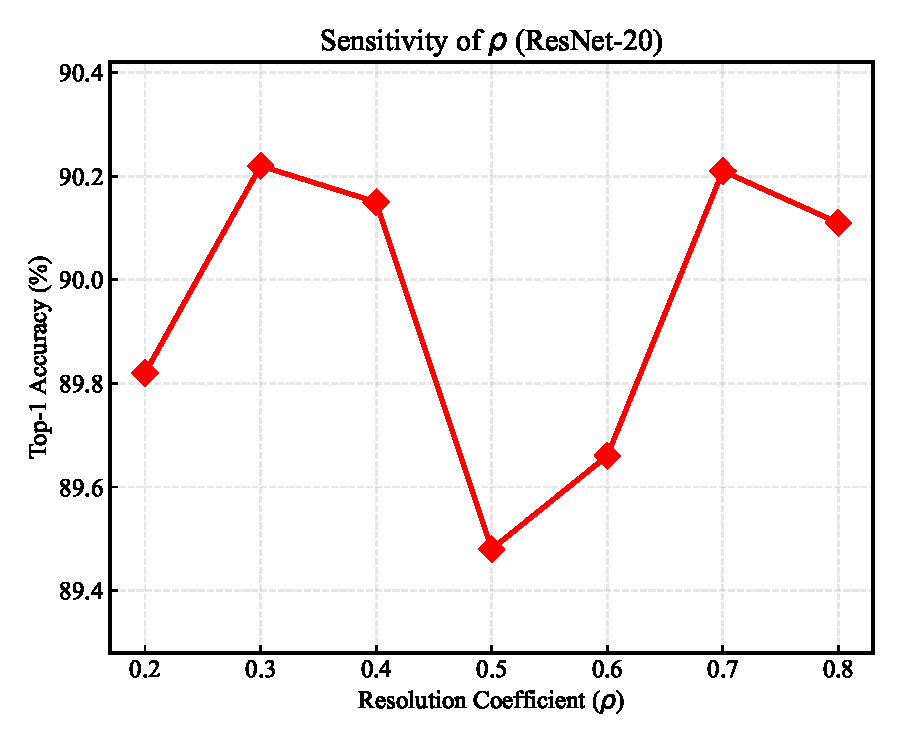
\includegraphics[width=0.85\textwidth]{fig7.pdf}
\caption{Sensitivity analysis of the resolution coefficient $\rho$ for GRA-CNN on ResNet-20. The method shows stable performance across a wide range of $\rho \in [0.3, 0.7]$, with the optimal trade-off observed at $\rho=0.5$.}
\label{fig:rho_ablation}
\end{figure*}
